\documentclass[12pt]{article}
\usepackage[margin=1in]{geometry} 
\usepackage{graphicx}
\usepackage{amsmath,amsthm,amssymb}
\usepackage{hyperref}

\title{
    \textbf{Programming Assignment 2} \\ 
    \textbf{CS5280} \\
}

\author{
    \textbf{Darpan Gaur} \\
    \textbf{CO21BTECH11004}
}


\date{}

\begin{document}
\maketitle

\hrulefill

\section*{Overview}
Implemented BTO, MVTO, MVTO-gc and k-MVTO using fine grained locking i.e., for operations read(), write() and tryCommmit() a lock on data-item is used, instead of a global lock.
For all experiments, $numIters=rand()\%500$ is taken instead of $numIters=rand()\%m$ as it was taking too long to run.

\section*{Number of transactions}
Parameters used to generate the data:
$n=16$, $m=1000$, $constVal=100$, $\lambda=20$, $readRatio=0.7$, $numTrans = [1000, 2000, 3000, 4000, 5000]$
% plot two figure side by side
\begin{figure*}[h]
    \centering
    \begin{minipage}[b]{0.45\textwidth}
        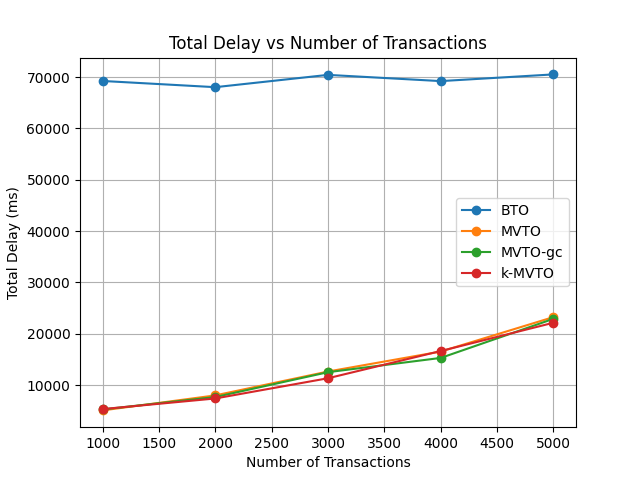
\includegraphics[width=\textwidth]{./images/NumTransTD.png}
        \caption{Commit Delay (BTO - MVTO)}
        \label{fig:numTransTD}
    \end{minipage}
    \hfill
    \begin{minipage}[b]{0.45\textwidth}
        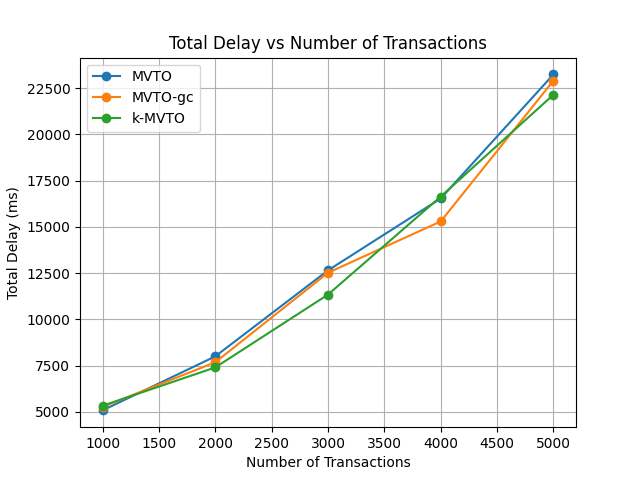
\includegraphics[width=\textwidth]{./images/MVTOnumTransTD.png}
        \caption{Commit Delay (MVTO)}
        \label{fig:MVTOnumTransTD}
    \end{minipage}
\end{figure*}\\
Figure \ref{fig:numTransTD} shows the commit delay for BTO and MVTO varients, while figure \ref{fig:MVTOnumTransTD} shows the commit delay for MVTO varients.
\begin{itemize}
    \item Commit delay for BTO is more than all MVTO varients, as there are more number of aborts in BTO than MVTO.
    \item Commit delay remains almost constant for BTO with increase in number of transactions.
    \item For MVTO varients commit delay increases with increase in number of transactions, as it takes more time to check to abort or commit a transaction.
    \item For MVTO-gc and k-MVTO, commit delay is slightly less than MVTO, due to garblage collection and limited versions respectively, which reduces the time for tryCommmit.
\end{itemize}
\begin{figure*}[h]
    \centering
    \begin{minipage}[b]{0.45\textwidth}
        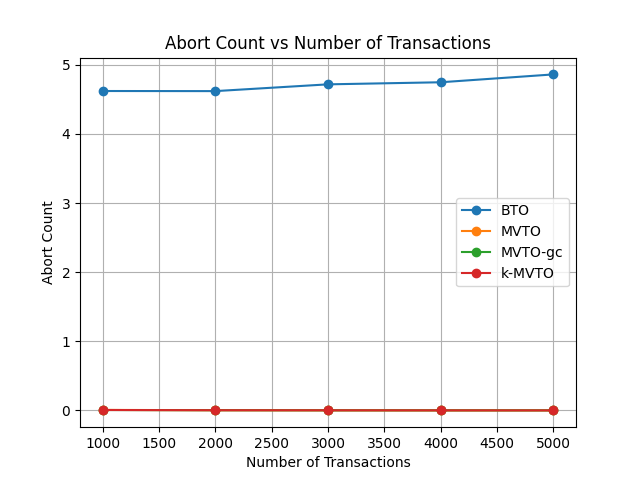
\includegraphics[width=\textwidth]{./images/NumTransAC.png}
        \caption{Abort Count (BTO - MVTO)}
        \label{fig:numTransAC}
    \end{minipage}
    \hfill
    \begin{minipage}[b]{0.45\textwidth}
        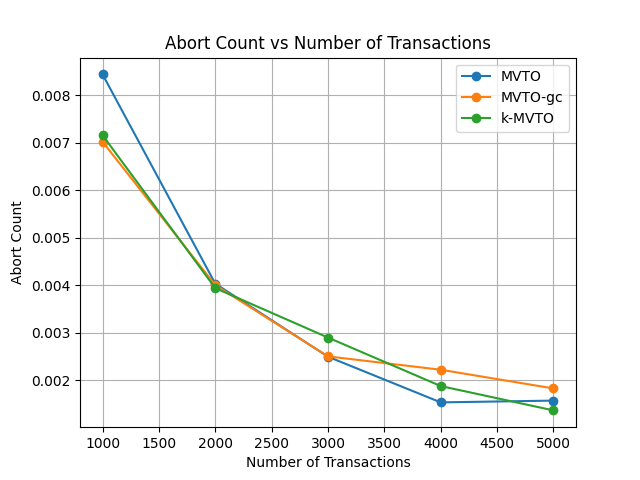
\includegraphics[width=\textwidth]{./images/MVTOnumTransAC.png}
        \caption{Abort Count (MVTO)}
        \label{fig:MVTOnumTransAC}
    \end{minipage}
\end{figure*}
Figure \ref{fig:numTransAC} shows the abort count for BTO and MVTO varients, while figure \ref{fig:MVTOnumTransAC} shows the abort count for MVTO varients.
\begin{itemize}
    \item Abort count for BTO is more than all MVTO varients, as we check with latest version.
    \item Abort count remains almost constant for BTO with increase in number of transactions.
    \item For MVTO varients abort count decreases with increase in number of transactions.
\end{itemize}

\section*{Number of variables}
Parameters used to generate the data:
$n=16$, $numTrans=1000$, $constVal=100$, $\lambda=20$, $readRatio=0.7$, $m = [1000, 2000, 3000, 4000, 5000]$.
\begin{figure*}[h]
    \centering
    \begin{minipage}[b]{0.45\textwidth}
        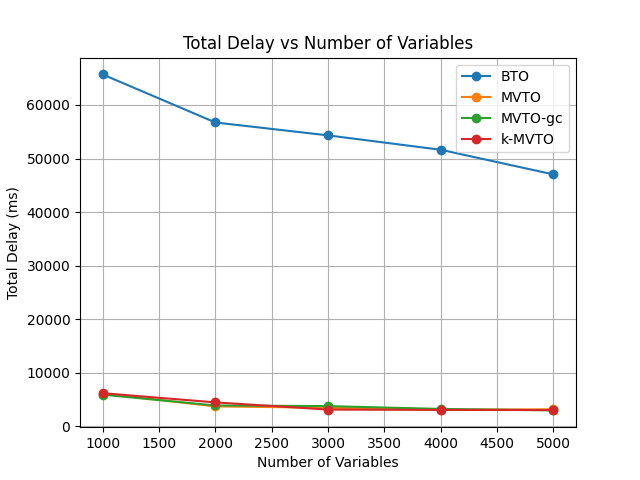
\includegraphics[width=\textwidth]{./images/VarTD.png}
        \caption{Commit Delay (BTO - MVTO)}
        \label{fig:varTD}
    \end{minipage}
    \hfill
    \begin{minipage}[b]{0.45\textwidth}
        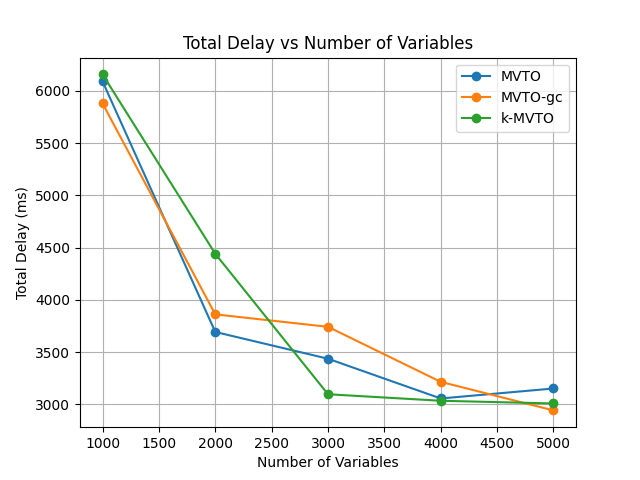
\includegraphics[width=\textwidth]{./images/MVTOvarTD.png}
        \caption{Commit Delay (MVTO)}
        \label{fig:MVTOvarTD}
    \end{minipage}
\end{figure*}\\
Figure \ref{fig:varTD} shows the commit delay for BTO and MVTO varients, while figure \ref{fig:MVTOvarTD} shows the commit delay for MVTO varients.
\begin{itemize}
    \item BTO has high commit delay than MVTO varients, as there are more number of aborts in BTO.
    \item For both BTO and MVTO varients, commit delay decreases with increase in number of variables, as less more variables less conflicts.
    \item For k-MVTO, commit delay is least as it has limited versions, which reduces the time for tryCommmit.
\end{itemize}
\begin{figure*}[h]
    \centering
    \begin{minipage}[b]{0.45\textwidth}
        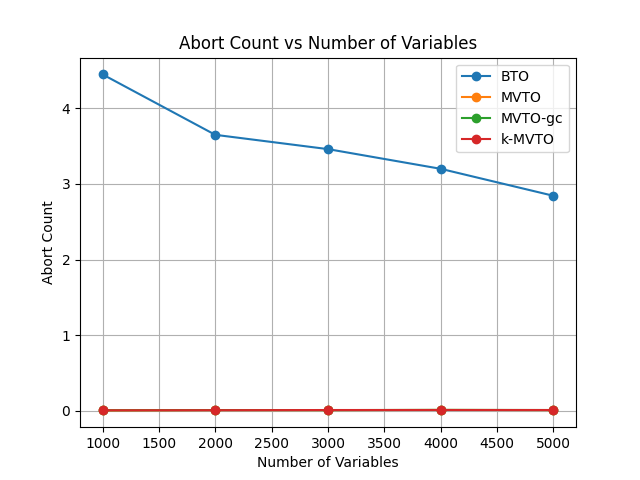
\includegraphics[width=\textwidth]{./images/VarAC.png}
        \caption{Abort Count (BTO - MVTO)}
        \label{fig:varAC}
    \end{minipage}
    \hfill
    \begin{minipage}[b]{0.45\textwidth}
        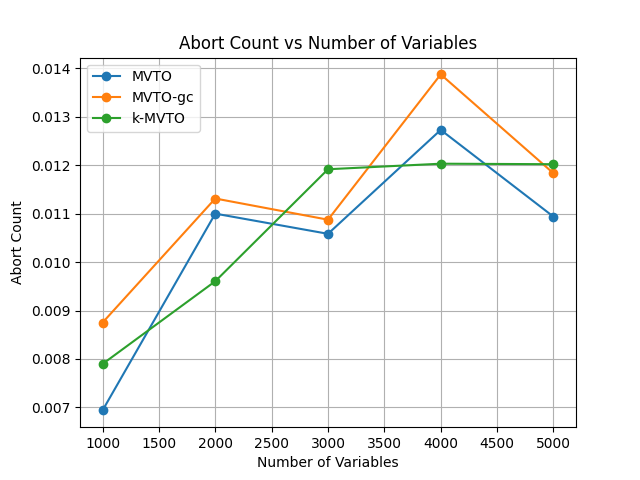
\includegraphics[width=\textwidth]{./images/MVTOvarAC.png}
        \caption{Abort Count (MVTO)}
        \label{fig:MVTOvarAC}
    \end{minipage}
\end{figure*}
Figure \ref{fig:varAC} shows the abort count for BTO and MVTO varients, while figure \ref{fig:MVTOvarAC} shows the abort count for MVTO varients.
\begin{itemize}
    \item Abort count for BTO is more than all MVTO varients, as we check with latest version.
    \item Abort count decreases with increase in number of variables for BTO, as less more variables less conflicts.
    \item For MVTO varients, abort count remains almost constant (slight increase) with increase in number of variables.
\end{itemize}

\section*{Number of threads}
Parameters used to generate the data:
$n=16$, $m=1000$, $numTrans=1000$, $constVal=100$, $\lambda=20$, $readRatio=0.7$, $numThreads = [2, 4, 8, 16, 32]$
\begin{figure*}[h]
    \centering
    \begin{minipage}[b]{0.45\textwidth}
        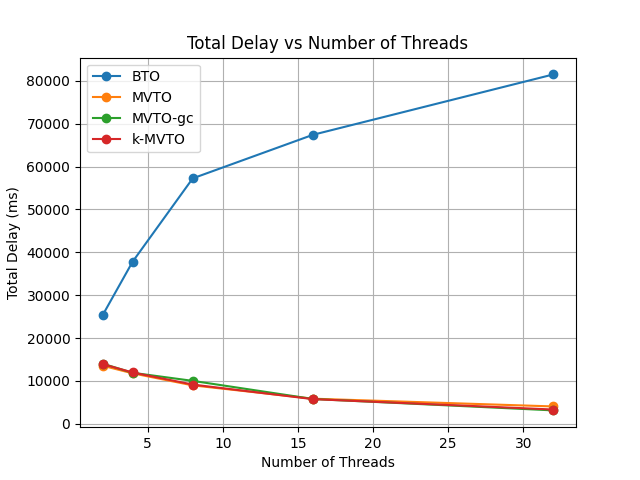
\includegraphics[width=\textwidth]{./images/ThreadsTD.png}
        \caption{Commit Delay (BTO - MVTO)}
        \label{fig:threadsTD}
    \end{minipage}
    \hfill
    \begin{minipage}[b]{0.45\textwidth}
        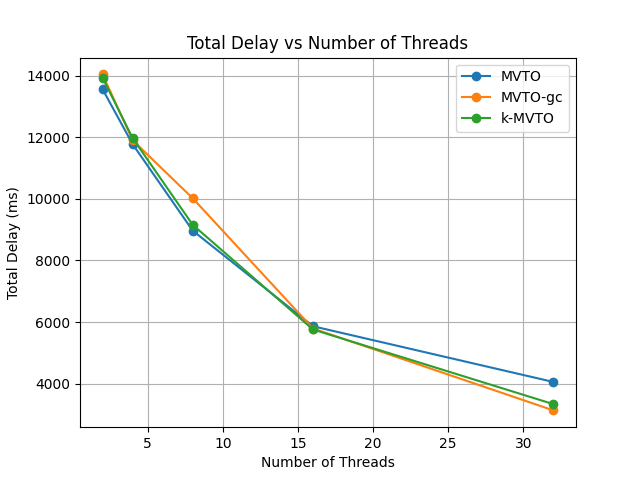
\includegraphics[width=\textwidth]{./images/MVTOThreadsTD.png}
        \caption{Commit Delay (MVTO)}
        \label{fig:MVTOThreadsTD}
    \end{minipage}
\end{figure*}\\
Figure \ref{fig:threadsTD} shows the commit delay for BTO and MVTO varients, while figure \ref{fig:MVTOThreadsTD} shows the commit delay for MVTO varients.
\begin{itemize}
    \item BTO has high commit delay than MVTO varients.
    \item For BTO commit delay increases with increase in number of threads, as more threads more conflicts.
    \item For MVTO varients, commit delay decreases with increase in number of threads, as more versions less conflicts.
\end{itemize}
\begin{figure*}[h]
    \centering
    \begin{minipage}[b]{0.45\textwidth}
        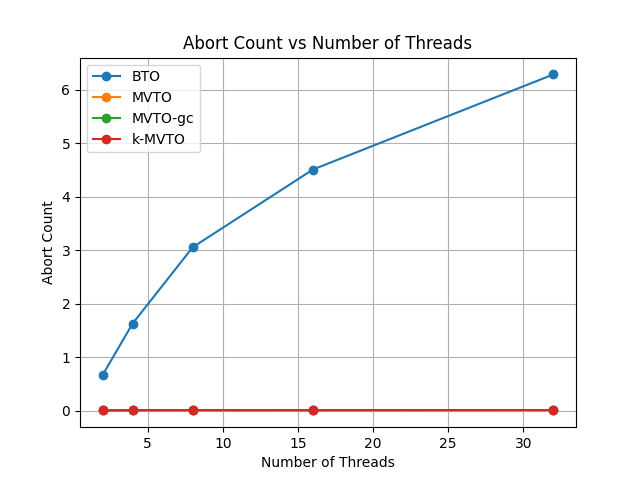
\includegraphics[width=\textwidth]{./images/ThreadsAC.png}
        \caption{Abort Count (BTO - MVTO)}
        \label{fig:threadsAC}
    \end{minipage}
    \hfill
    \begin{minipage}[b]{0.45\textwidth}
        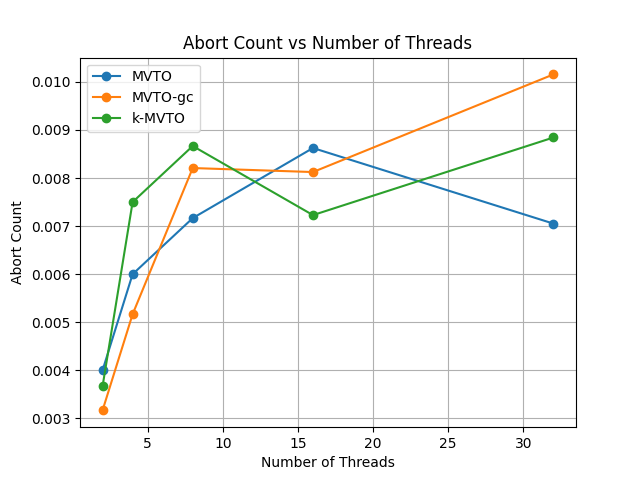
\includegraphics[width=\textwidth]{./images/MVTOThreadsAC.png}
        \caption{Abort Count (MVTO)}
        \label{fig:MVTOThreadsAC}
    \end{minipage}
\end{figure*}
\begin{itemize}
    \item Abort count for BTO is more than all MVTO varients.
    \item Abort count increases with increase in number of threads for BTO, as more threads more conflicts.
    \item For MVTO varients, abort count remains almost constant (slight increase) with increase in number of threads.
\end{itemize}

\section*{K for K-MVTO}
Parameters used to generate the data:
$n=16$, $m=1000$, $numTrans=1000$, $constVal=100$, $\lambda=20$, $readRatio$, $K = [5, 10, 15, 20, 25]$
\begin{figure*}[h]
    \centering
    \begin{minipage}[b]{0.45\textwidth}
        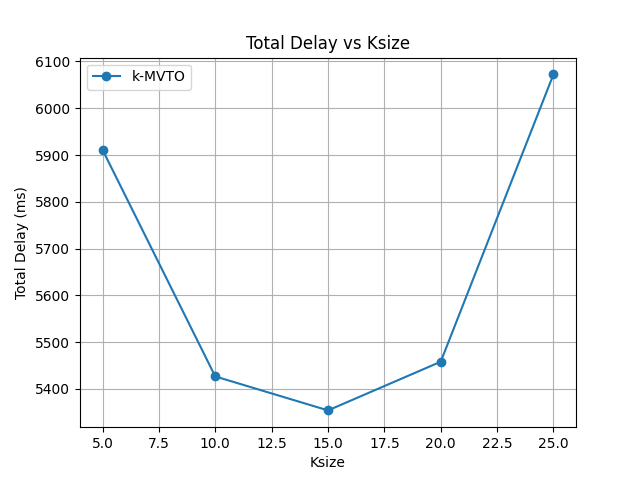
\includegraphics[width=\textwidth]{./images/KsizeTD.png}
        \caption{Commit Delay (BTO-MVTO)}
        \label{fig:KsizeTD}
    \end{minipage}
    \hfill
    \begin{minipage}[b]{0.45\textwidth}
        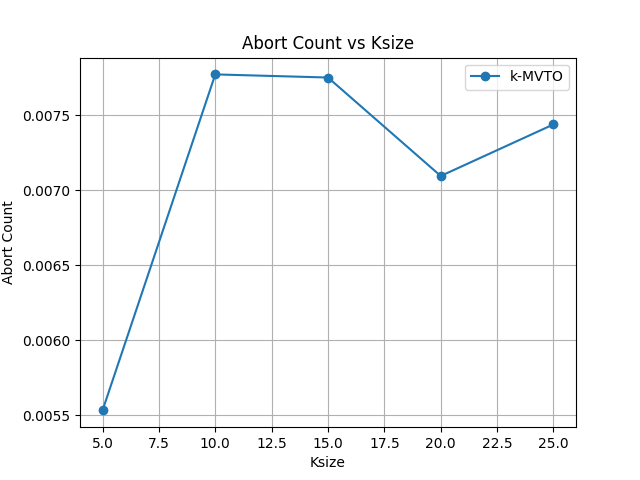
\includegraphics[width=\textwidth]{./images/KsizeAC.png}
        \caption{Abort Count (BTO-MVTO)}
        \label{fig:KsizeAC}
    \end{minipage}
\end{figure*}\\
\begin{itemize}
    \item Total delay first decreases and then increases with increase in K.
    \item Abort count reamins constant (slight increase) with increase in K.
\end{itemize}

\section*{Read Ratio}
Parameters used to generate the data:
$n=16$, $m=1000$, $numTrans=1000$, $constVal=100$, $\lambda=20$, $readRatio = [0.5, 0.6, 0.7, 0.8, 0.9]$
\begin{figure*}[h]
    \centering
    \begin{minipage}[b]{0.45\textwidth}
        \includegraphics[width=\textwidth]{./images/ReadRatioTD.png}
        \caption{Commit Delay (BTO-MVTO)}
        \label{fig:ReadRatioTD}
    \end{minipage}
    \hfill
    \begin{minipage}[b]{0.45\textwidth}
        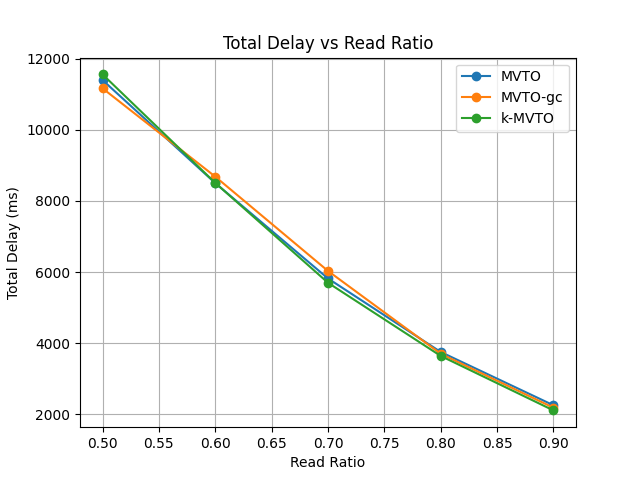
\includegraphics[width=\textwidth]{./images/MVTOreadRatioTD.png}
        \caption{Commit Delay (MVTO)}
        \label{fig:MVTOreadRatioTD}
    \end{minipage}
\end{figure*} \\
\begin{itemize}
    \item Commit delay for BTO is more than all MVTO varients, as there are more number of aborts in BTO.
    \item Commit delay decreases with increase in read ratio for both BTO and MVTO varients, as more reads less conflicts.
\end{itemize}
\begin{figure*}[h]
    \centering
    \begin{minipage}[b]{0.45\textwidth}
        \includegraphics[width=\textwidth]{./images/ReadRatioAC.png}
        \caption{Abort Count (BTO-MVTO)}
        \label{fig:ReadRatioAC}
    \end{minipage}
    \hfill
    \begin{minipage}[b]{0.45\textwidth}
        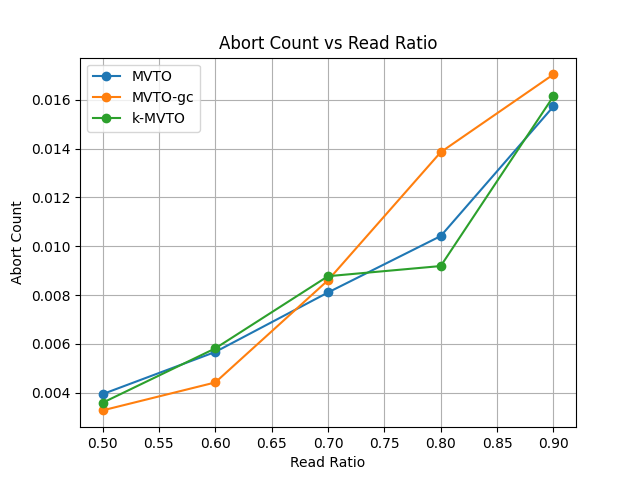
\includegraphics[width=\textwidth]{./images/MVTOreadRatioAC.png}
        \caption{Abort Count (MVTO)}
        \label{fig:MVTOreadRatioAC}
    \end{minipage}
\end{figure*}
\begin{itemize}
    \item Abort count for BTO is more than all MVTO varients, as we check with latest version.
    \item Abort count decreases with increase in read ratio for BTO, as more reads less conflicts.
    \item For MVTO varients, abort count remains almost constant (slight increase) with increase in read ratio.
\end{itemize}
\end{document}